\section* {3.1. Построение интерполяционных многочленов Лагранжа и Ньютона}


\subsection{Постановка задачи}
Используя таблицу значений $Y_i$ функции $y = f(x)$, вычисленных в точках $X_i, i = 0, ..., 3$ построить интерполяционные многочлены Лагранжа и Ньютона, проходящие через точки $\{X_i, Y_i\}$.  Вычислить значение погрешности интерполяции в точке $X_i$. 

{\bfseries Вариант:} 5
\begin{align*}
& y = ln(x), \\
& a) X_i = 0.2, 0.6, 1.0, 1.4;\\
& b) X_i = 0.2, 0.6, 1.0, 1.4;\\
& X^* = 0.8 \\
\end{align*}

\subsection{Результаты работы}
\begin{figure}[h!]
\centering
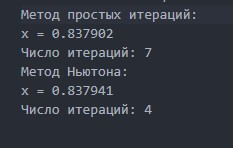
\includegraphics[width=.9\textwidth]{img1}
\end{figure}

\subsection{Исходный код}
\lstinputlisting{include/task_3_1.cpp}
\pagebreak

\section* {3.2. Построение кубического сплайна для функции, заданной в узлах интерполяции}

\setcounter{subsection}{0}


\subsection{Постановка задачи}
Построить кубический сплайн для функции, заданной в узлах интерполяции, предполагая, что сплайн имеет нулевую кривизну при $x = x_0$ и $x = x_4$. Вычислить значение функции в точке $x = X^*$.  

{\bfseries Вариант:} 5
\begin{align*}
& X^* = 0.8, \\
& x_i = \{0.1, 0.5, 0.9, 1.3, 1.7\}, \\
& y_i = \{-2.3026, -0.69315, -0.10536, 0.26236, 0.53063\} \\
\end{align*}

\subsection{Результаты работы}
\begin{figure}[h!]
\centering
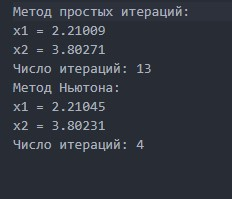
\includegraphics[width=.9\textwidth]{img2}
\end{figure}
\pagebreak

\subsection{Исходный код}
\lstinputlisting{include/task_3_2.cpp}
\pagebreak

\section* {3.3. Нахождение приближающих многочленов таблично заданной функции}

\setcounter{subsection}{0}


\subsection{Постановка задачи}
Для таблично заданной функции путем решения нормальной системы МНК найти приближающие многочлены a) 1-ой  и б) 2-ой степени. Для каждого из приближающих многочленов вычислить сумму квадратов ошибок. Построить графики приближаемой функции и приближающих многочленов.  

{\bfseries Вариант:} 5
\begin{align*}
& x_i = \{0.1, 0.5, 0.9, 1.3, 1.7, 2.1\}, \\
& y_i = \{-2.3026, -0.69315, -0.10536, 0.26236, 0.53063, 0.74194\} \\
\end{align*}

\subsection{Результаты работы}
\begin{figure}[h!]
\centering
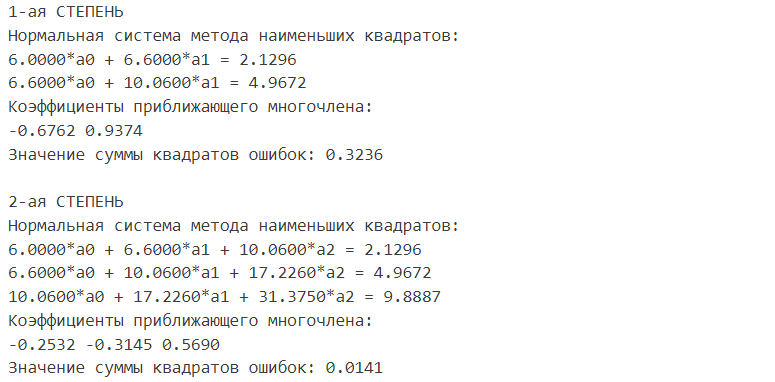
\includegraphics[width=.9\textwidth]{img3}
\end{figure}
\pagebreak

\subsection{Исходный код}
\lstinputlisting{include/task_3_3.cpp}
\pagebreak

\section* {3.4. Вычисление производных таблично заданной функции}

\setcounter{subsection}{0}


\subsection{Постановка задачи}
Вычислить первую и вторую производную от таблично заданной функции $y_i = f(x_i), i = 0, 1, 2, 3, 4$ в точке $x = X^*$.  

{\bfseries Вариант:} 5
\begin{align*}
& X^* = 2.0 \\
& x_i = \{0.0, 1.0, 2.0, 3.0, 4.0\}, \\
& y_i = \{0.0, 1.0, 1.4142, 1.7321, 2.0\} \\
\end{align*}

\subsection{Результаты работы}
\begin{figure}[h!]
\centering
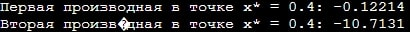
\includegraphics[width=.9\textwidth]{img4}
\end{figure}
\pagebreak

\subsection{Исходный код}
\lstinputlisting{include/task_3_4.cpp}
\pagebreak

\section* {3.5. Вычисление определённого интеграла методами прямоугольников, трапеций и Симпсона}

\setcounter{subsection}{0}


\subsection{Постановка задачи}
Вычислить определенный интеграл $F = \int_{X_0}^{X_1} y dx$, методами прямоугольников, трапеций, Симпсона с шагами $h_1, h_2$. Оценить погрешность вычислений, используя  Метод Рунге-Ромберга.  

{\bfseries Вариант:} 5
\begin{align*}
& y = \frac{1}{(2x + 7)(3x + 4)}, \\
& X_0 = -1, X_k = 1, h_1 = 0.5, h_2 = 0.25 \\
\end{align*}

\subsection{Результаты работы}
\begin{figure}[h!]
\centering
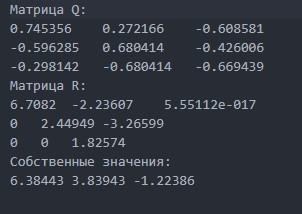
\includegraphics[width=.9\textwidth]{img5}
\end{figure}
\pagebreak

\subsection{Исходный код}
\lstinputlisting{include/task_3_5.cpp}
\pagebreak